\documentclass[border=3pt,tikz]{standalone}
\usepackage{amsmath,amssymb}
\usepackage{bm} % math bold
\usepackage{tikz}
\usetikzlibrary{patterns}
\tikzset{>=latex}

\colorlet{myblue}{black!50!blue}
\colorlet{mygreen}{black!50!green}
\colorlet{myred}{black!50!red}

\begin{document}


% RESISTANCE vs. TEMPERATURE
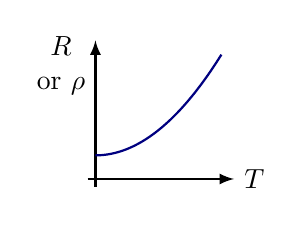
\begin{tikzpicture}
  \def\N{20}
  \def\xmin{-0.1} \def\xmax{1.6}
  \def\ymin{-0.1} \def\ymax{1.6}
  \draw[->,thick]
    (\xmin,0) -- (1.1*\xmax,0) node[right] {$T$};
  \draw[->,thick]
    (0,\ymin) -- (0,1.1*\ymax) node[above=5pt,below left,align=center] {$R$\\ or $\rho$};  
  \draw[thick,myblue,variable=\x,domain=0:\xmax,samples=\N,smooth]
    plot (\x,0.3+\x*\x/2);
\end{tikzpicture}


% TEMPERATURE SCALE
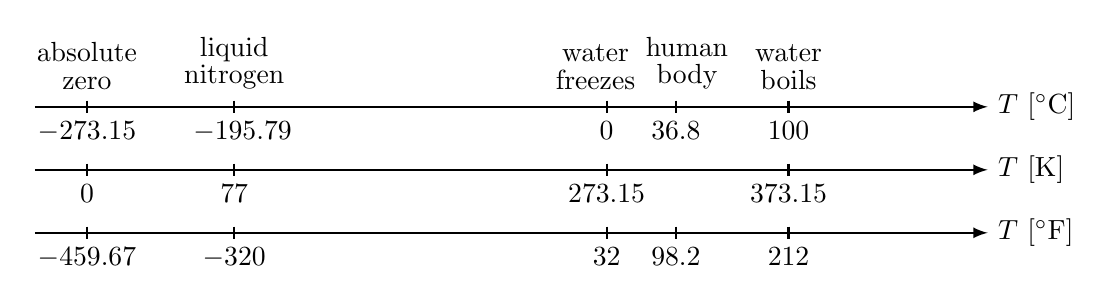
\begin{tikzpicture}[xscale=1.1]
  \def\Tzero{-6.0}
  \def\Tmax{4.0}
  \def\Tnitro{-4.3}
  \def\Tbody{0.8}
  \def\Tboil{2.1}
  \def\tick#1#2{\draw[thick] (#1+.08) --++ (0,-.16) node[below=-.5pt,scale=1] {#2};}
  
  % AXIS
  \draw[->,thick]
    (1.1*\Tzero,0) -- (1.1*\Tmax,0) node[right] {$T$ [$^\circ$C]};
  \draw[->,thick]
    (1.1*\Tzero,-.8) -- (1.1*\Tmax,-.8) node[right] {$T$ [K]};
  \draw[->,thick]
    (1.1*\Tzero,-1.6) -- (1.1*\Tmax,-1.6) node[right] {$T$ [$^\circ$F]};
  
  % LABEL
  \node[above,align=center] at (\Tzero,0.1) {absolute\\[-2] zero};
  \node[above,align=center] at (\Tnitro,0.1) {liquid\\[-2] nitrogen};
  \node[left=4,above,align=center] at (0,0.1) {water\\[-2] freezes};
  \node[right=4,above,align=center] at (\Tbody,0.1) {human\\[-2] body};
  \node[above,align=center] at (\Tboil,0.1) {water\\[-2] boils};
  
  % CELSIUS
  \tick{\Tzero,0}{$-273.15$}
  \tick{\Tnitro,0}{\hspace{6pt}$-195.79$}
  \tick{0,0}{0}
  \tick{\Tbody,0}{36.8}
  \tick{\Tboil,0}{100}
  
  % KELVIN
  \tick{\Tzero,-.8}{0}
  \tick{\Tnitro,-.8}{77}
  \tick{0,-.8}{273.15}
  \tick{\Tboil,-.8}{373.15}
  
  % FAHRENHEIT
  \tick{\Tzero,-1.6}{$-459.67$} 
  \tick{\Tnitro,-1.6}{$-320$}
  \tick{0,-1.6}{32}
  \tick{\Tbody,-1.6}{98.2}
  \tick{\Tboil,-1.6}{212}
  
\end{tikzpicture}


% PRESSURE vs. TEMPERATURE
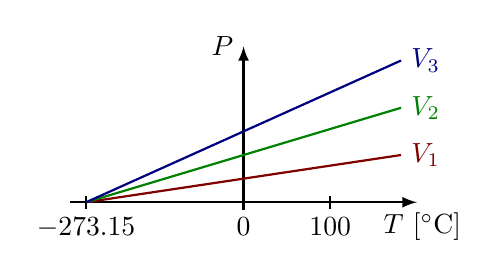
\begin{tikzpicture}
  \def\xmin{-2.0} \def\xmax{2.0}
  \def\ymin{-0.1} \def\ymax{1.8}
  \def\tick#1#2{\draw[thick] (#1+.08) --++ (0,-.16) node[below=-.5pt] {#2};}
  
  % AXIS
  \draw[->,thick]
    (1.1*\xmin,0) -- (1.1*\xmax,0) node[right=2,below] {$T$ [$^\circ$C]};
  \draw[->,thick]
    (0,\ymin) -- (0,1.1*\ymax) node[left,align=center] {$P$};
  
  % TICK
  \tick{\xmin,0}{$-273.15$}
  \tick{0,0}{0}
  \tick{1.1,0}{100}
  
  % GAS LINE
  \draw[thick,myred] (\xmin,0) -- (\xmax,0.6) node[right] {$V_1$};
  \draw[thick,mygreen] (\xmin,0) -- (\xmax,1.2) node[right] {$V_2$};
  \draw[thick,myblue] (\xmin,0) -- (\xmax,1.8) node[right] {$V_3$};
  
\end{tikzpicture}


% PRESSURE vs. VOLUME
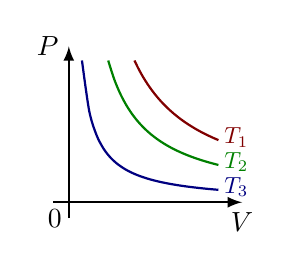
\begin{tikzpicture}
  \def\N{20}
  \def\nRTr{1.5}
  \def\nRTg{0.9}
  \def\nRTb{0.3}
  \def\xmax{2.0}
  \def\ymax{1.8}
  \def\tick#1#2{\draw[thick] (#1+.08) --++ (0,-.16) node[below=-.5pt] {#2};}
  
  % AXIS
  \draw[->,thick]
    (-0.1*\xmax,0) -- (1.1*\xmax,0) node[below] {$V$}; % [$\text{m}^3$]};
  \draw[->,thick]
    (0,-0.1*\xmax) -- (0,1.1*\ymax) node[left,align=center] {$P$};
  \node[below left=-1] at (0,0) {0};
  
  % ISOTHERMS
  \draw[thick,myred,variable=\x,domain=\nRTr/\ymax:0.95*\xmax,samples=\N,smooth]
    plot (\x,\nRTr/\x) node[above=1,right=-1,scale=0.84] {$T_1$};
  \draw[thick,mygreen,variable=\x,domain=\nRTg/\ymax:0.95*\xmax,samples=\N,smooth]
    plot (\x,\nRTg/\x) node[above=1,right=-1,scale=0.84] {$T_2$};
  \draw[thick,myblue,variable=\x,domain=\nRTb/\ymax:0.95*\xmax,samples=\N,smooth]
    plot (\x,\nRTb/\x) node[above=1,right=-1,scale=0.84] {$T_3$};
  
\end{tikzpicture}



\end{document}
